\chapter{Verkkojen perusteet}
Monen ohjelmointitehtävän voi ratkaista tulkitsemalla
tehtävän verkko-on\-gel\-ma\-na ja käyttämällä
sopivaa verkkoalgoritmia.
Tyypillinen esimerkki verkosta on tieverkosto,
jonka rakenne muistuttaa luonnostaan verkkoa.
Joskus taas verkko kätkeytyy syvemmälle ongelmaan
ja sitä voi olla vaikeaa huomata.

Tässä kirjan osassa tutustumme verkkojen käsittelyyn
liittyviin tekniikoihin ja kisakoodauksessa
keskeisiin verkkoalgoritmeihin.
Aloitamme aiheeseen perehtymisen
käymällä läpi verkkoihin liittyviä käsitteitä
sekä erilaisia tapoja pitää verkkoa muistissa algoritmeissa.

\section{Käsitteitä}

Verkko (\textit{graph})
muodostuu solmuista (\textit{node} tai \textit{vertex})
ja niiden välisistä kaarista (\textit{edge}).
Merkitsemme tässä kirjassa yleensä
verkon solmujen määrää
muuttujalla $n$ ja verkon kaarten määrää muuttujalla $m$.
Lisäksi numeroimme verkon solmut kokonaisluvuin
$1,2,\ldots,n$.

Esimerkiksi seuraavassa verkossa on 5 solmua ja 7 kaarta:

\begin{center}
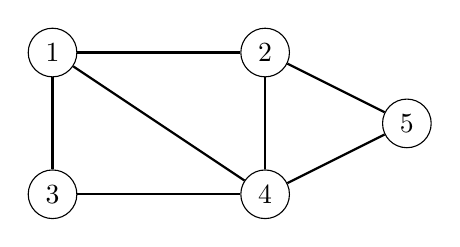
\begin{tikzpicture}[scale=0.9]
\node[draw, circle] (1) at (1,3) {$1$};
\node[draw, circle] (2) at (4,3) {$2$};
\node[draw, circle] (3) at (1,1) {$3$};
\node[draw, circle] (4) at (4,1) {$4$};
\node[draw, circle] (5) at (6,2) {$5$};

\path[draw,thick,-] (1) -- (2);
\path[draw,thick,-] (1) -- (3);
\path[draw,thick,-] (1) -- (4);
\path[draw,thick,-] (3) -- (4);
\path[draw,thick,-] (2) -- (4);
\path[draw,thick,-] (2) -- (5);
\path[draw,thick,-] (4) -- (5);
\end{tikzpicture}
\end{center}

Polku (\textit{path}) on solmusta $a$ solmuun $b$
johtava reitti, joka kulkee verkon kaaria pitkin.
Polun pituus (\textit{length}) on kaarten määrä polulla.
Esimerkiksi yllä olevassa verkossa
mahdollisia polkuja solmusta 1 solmuun 5 ovat:

\begin{itemize}
\item $1 \rightarrow 2 \rightarrow 5$ (pituus 2)
\item $1 \rightarrow 4 \rightarrow 5$ (pituus 2)
\item $1 \rightarrow 2 \rightarrow 4 \rightarrow 5$ (pituus 3)
\item $1 \rightarrow 3 \rightarrow 4 \rightarrow 5$ (pituus 3)
\item $1 \rightarrow 3 \rightarrow 4 \rightarrow 2 \rightarrow 5$ (pituus 4)
\end{itemize}

\subsubsection{Yhtenäisyys}

Verkko on yhtenäinen (\textit{connected}), jos siinä on polku
mistä tahansa solmusta mihin tahansa solmuun.
Esimerkiksi seuraava verkko on yhtenäinen:
\begin{center}
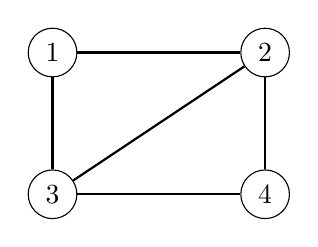
\begin{tikzpicture}[scale=0.9]
\node[draw, circle] (1) at (1,3) {$1$};
\node[draw, circle] (2) at (4,3) {$2$};
\node[draw, circle] (3) at (1,1) {$3$};
\node[draw, circle] (4) at (4,1) {$4$};
\path[draw,thick,-] (1) -- (2);
\path[draw,thick,-] (1) -- (3);
\path[draw,thick,-] (2) -- (3);
\path[draw,thick,-] (3) -- (4);
\path[draw,thick,-] (2) -- (4);
\end{tikzpicture}
\end{center}

Seuraava verkko taas ei ole yhtenäinen,
koska esimerkiksi solmusta 1 ei ole polkua solmuun 2.
\begin{center}
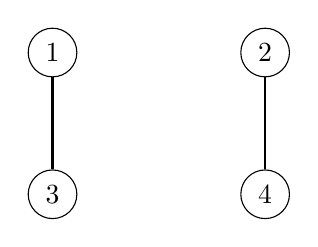
\begin{tikzpicture}[scale=0.9]
\node[draw, circle] (1) at (1,3) {$1$};
\node[draw, circle] (2) at (4,3) {$2$};
\node[draw, circle] (3) at (1,1) {$3$};
\node[draw, circle] (4) at (4,1) {$4$};
%\path[draw,thick,-] (1) -- (2);
\path[draw,thick,-] (1) -- (3);
%\path[draw,thick,-] (2) -- (3);
%\path[draw,thick,-] (3) -- (4);
\path[draw,thick,-] (2) -- (4);
\end{tikzpicture}
\end{center}

Verkon yhtenäiset osat muodostavat sen
komponentit (\textit{components}).
Esimerkiksi seuraavassa verkossa on
kolme komponenttia:
$\{1,\,2,\,3\}$,
$\{4,\,5,\,6,\,7\}$ ja
$\{8\}$.
\begin{center}
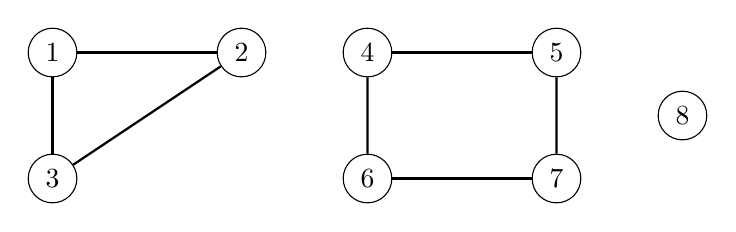
\begin{tikzpicture}[scale=0.8]
\node[draw, circle] (1) at (1,3) {$1$};
\node[draw, circle] (2) at (4,3) {$2$};
\node[draw, circle] (3) at (1,1) {$3$};

\node[draw, circle] (6) at (6,1) {$6$};
\node[draw, circle] (7) at (9,1) {$7$};
\node[draw, circle] (4) at (6,3) {$4$};
\node[draw, circle] (5) at (9,3) {$5$};

\node[draw, circle] (8) at (11,2) {$8$};

\path[draw,thick,-] (1) -- (2);
\path[draw,thick,-] (2) -- (3);
\path[draw,thick,-] (1) -- (3);
\path[draw,thick,-] (4) -- (5);
\path[draw,thick,-] (5) -- (7);
\path[draw,thick,-] (6) -- (7);
\path[draw,thick,-] (6) -- (4);
\end{tikzpicture}
\end{center}

Puu (\textit{tree}) on yhtenäinen verkko,
jossa on $n$ solmua ja $n-1$ kaarta.
Siinä jokaisen solmun välillä on yksikäsitteinen polku,
ja jos minkä tahansa kaaren poistaa,
verkko ei ole enää yhtenäinen.
Esimerkiksi seuraava verkko on puu:

\begin{center}
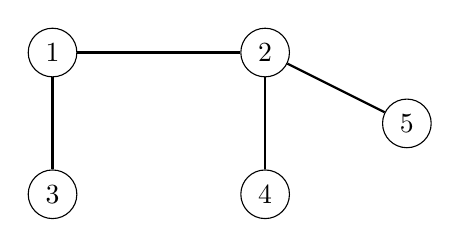
\begin{tikzpicture}[scale=0.9]
\node[draw, circle] (1) at (1,3) {$1$};
\node[draw, circle] (2) at (4,3) {$2$};
\node[draw, circle] (3) at (1,1) {$3$};
\node[draw, circle] (4) at (4,1) {$4$};
\node[draw, circle] (5) at (6,2) {$5$};

\path[draw,thick,-] (1) -- (2);
\path[draw,thick,-] (1) -- (3);
%\path[draw,thick,-] (1) -- (4);
\path[draw,thick,-] (2) -- (5);
\path[draw,thick,-] (2) -- (4);
%\path[draw,thick,-] (4) -- (5);
\end{tikzpicture}
\end{center}

\subsubsection{Kaarten suunnat}

Verkko on suunnattu (\textit{directed}),
jos verkon kaaria pystyy
kulkemaan vain niiden merkittyyn suuntaan.
Esimerkiki seuraava verkko on suunnattu:
\begin{center}
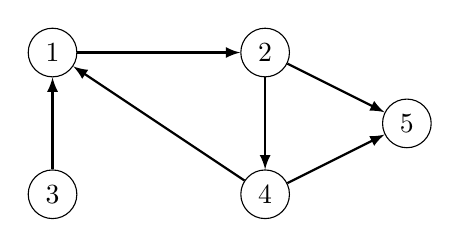
\begin{tikzpicture}[scale=0.9]
\node[draw, circle] (1) at (1,3) {$1$};
\node[draw, circle] (2) at (4,3) {$2$};
\node[draw, circle] (3) at (1,1) {$3$};
\node[draw, circle] (4) at (4,1) {$4$};
\node[draw, circle] (5) at (6,2) {$5$};
\path[draw,thick,->,>=latex] (1) -- (2);
\path[draw,thick,->,>=latex] (2) -- (4);
\path[draw,thick,->,>=latex] (2) -- (5);
\path[draw,thick,->,>=latex] (4) -- (5);
\path[draw,thick,->,>=latex] (4) -- (1);
\path[draw,thick,->,>=latex] (3) -- (1);
\end{tikzpicture}
\end{center}

Yllä olevassa verkossa solmusta 3 on polku
kaikkiin muihin verkon solmuihin.
Esimerkiksi solmusta 3 pääsee solmuun 5 pääsee polkua
$3 \rightarrow 1 \rightarrow 2 \rightarrow 5$.
Sen sijaan solmusta 5 ei lähde polkua mihinkään muuhun
solmuun.

Suunnattu verkko on vahvasti yhtenäinen
(\textit{strongly connected}),
jos mistä tahansa solmusta on polku mihin
tahansa toiseen solmuun.

Sykli (\textit{cycle}) on polku, jonka ensimmäinen
ja viimeinen solmu on sama.
Esimerkiksi yllä olevassa verkossa on sykli
$1 \rightarrow 2 \rightarrow 4 \rightarrow 1$.
Jos verkossa ei ole yhtään sykliä, se on syklitön
(\textit{acyclic}).

\subsubsection{Kaarten painot}

Painotetussa (\textit{weighted}) verkossa
jokaisesta kaaresta tiedetään sen paino.
Tavallinen tulkinta on, että painot kuvaavat
kaarien pituuksia.
Seuraavassa on esimerkki painotetusta verkosta:
\begin{center}
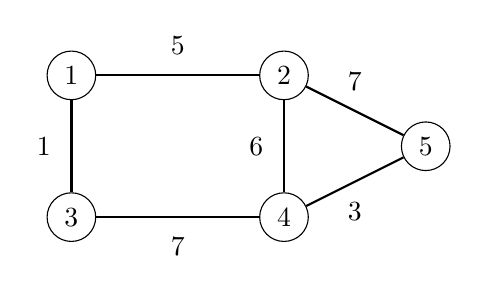
\begin{tikzpicture}[scale=0.9]
\node[draw, circle] (1) at (1,3) {$1$};
\node[draw, circle] (2) at (4,3) {$2$};
\node[draw, circle] (3) at (1,1) {$3$};
\node[draw, circle] (4) at (4,1) {$4$};
\node[draw, circle] (5) at (6,2) {$5$};
\path[draw,thick,-] (1) -- node[font=\small,label=above:5] {} (2);
\path[draw,thick,-] (1) -- node[font=\small,label=left:1] {} (3);
\path[draw,thick,-] (3) -- node[font=\small,label=below:7] {} (4);
\path[draw,thick,-] (2) -- node[font=\small,label=left:6] {} (4);
\path[draw,thick,-] (2) -- node[font=\small,label=above:7] {} (5);
\path[draw,thick,-] (4) -- node[font=\small,label=below:3] {} (5);
\end{tikzpicture}
\end{center}

Painotetussa verkossa polun pituus on sen kaarten painojen summa.
Esimerkiksi polun $1 \rightarrow 2 \rightarrow 5$
pituus on $5+7=12$ ja polun
$1 \rightarrow 3 \rightarrow 4 \rightarrow 5$ pituus on $1+7+3=11$.
Jälkimmäinen polku on lyhin polku solmusta 1 solmuun 5.

\subsubsection{Naapurit ja asteet}

Kaksi solmua ovat naapureita (\textit{neighbor}),
jos ne ovat vierekkäin eli niiden välillä on kaari.
Solmun aste (\textit{degree}) on
sen naapurien määrä.
Esimerkiksi seuraavassa verkossa
solmun 2 naapurit ovat 1, 4 ja 5,
joten sen aste on 3.

\begin{center}
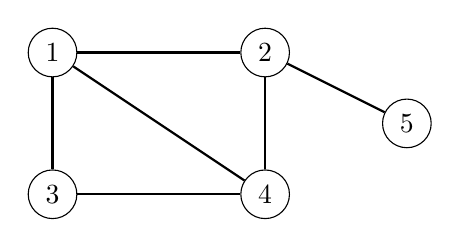
\begin{tikzpicture}[scale=0.9]
\node[draw, circle] (1) at (1,3) {$1$};
\node[draw, circle] (2) at (4,3) {$2$};
\node[draw, circle] (3) at (1,1) {$3$};
\node[draw, circle] (4) at (4,1) {$4$};
\node[draw, circle] (5) at (6,2) {$5$};

\path[draw,thick,-] (1) -- (2);
\path[draw,thick,-] (1) -- (3);
\path[draw,thick,-] (1) -- (4);
\path[draw,thick,-] (3) -- (4);
\path[draw,thick,-] (2) -- (4);
\path[draw,thick,-] (2) -- (5);
%\path[draw,thick,-] (4) -- (5);
\end{tikzpicture}
\end{center}

Verkon solmujen asteiden summa on $2m$,
missä $m$ on kaarten määrä.
Tämä johtuu siitä, että jokainen kaari lisää
kahden solmun astetta yhdellä.
Niinpä solmujen asteiden summa on aina parillinen.

Verkko on säännöllinen (\textit{regular}),
jos jokaisen solmun aste on vakio $d$.
Verkko on täydellinen (\textit{complete}),
jos jokaisen solmun aste on $n-1$ eli
verkossa on kaikki mahdolliset kaaret
solmujen välillä.

Suunnatussa verkossa lähtöaste (\textit{outdegree})
on solmusta lähtevien kaarten määrä ja
tuloaste (\textit{indegree}) on solmuun tulevien
kaarten määrä.
Esimerkiksi seuraavassa verkossa solmun 2
lähtöaste on 1 ja tuloaste on 2.

\begin{center}
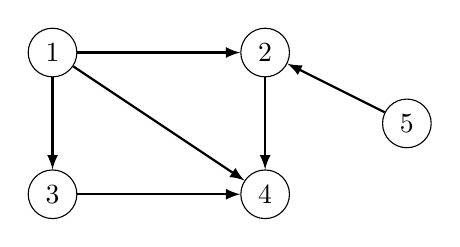
\begin{tikzpicture}[scale=0.9]
\node[draw, circle] (1) at (1,3) {$1$};
\node[draw, circle] (2) at (4,3) {$2$};
\node[draw, circle] (3) at (1,1) {$3$};
\node[draw, circle] (4) at (4,1) {$4$};
\node[draw, circle] (5) at (6,2) {$5$};

\path[draw,thick,->,>=latex] (1) -- (2);
\path[draw,thick,->,>=latex] (1) -- (3);
\path[draw,thick,->,>=latex] (1) -- (4);
\path[draw,thick,->,>=latex] (3) -- (4);
\path[draw,thick,->,>=latex] (2) -- (4);
\path[draw,thick,<-,>=latex] (2) -- (5);
\end{tikzpicture}
\end{center}

\subsubsection{Väritykset}

Verkon värityksessä (\textit{coloring}) jokaiselle solmulle valitaan
tietty väri niin, että millään kahdella
vierekkäisellä solmulla ei ole samaa väriä.
Verkko on kaksijakoinen (\textit{bipartite}),
jos kaksi väriä riittää sen värittämiseen.

Esimerkiksi verkko
\begin{center}
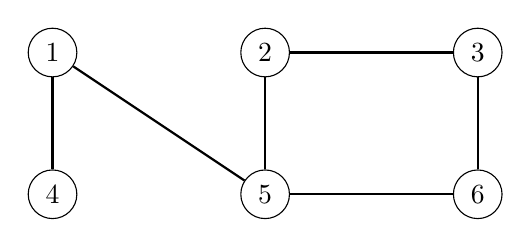
\begin{tikzpicture}[scale=0.9]
\node[draw, circle] (1) at (1,3) {$2$};
\node[draw, circle] (2) at (4,3) {$3$};
\node[draw, circle] (3) at (1,1) {$5$};
\node[draw, circle] (4) at (4,1) {$6$};
\node[draw, circle] (5) at (-2,1) {$4$};
\node[draw, circle] (6) at (-2,3) {$1$};
\path[draw,thick,-] (1) -- (2);
\path[draw,thick,-] (1) -- (3);
\path[draw,thick,-] (3) -- (4);
\path[draw,thick,-] (2) -- (4);
\path[draw,thick,-] (3) -- (6);
\path[draw,thick,-] (5) -- (6);
\end{tikzpicture}
\end{center}
on kaksijakoinen, koska sen voi värittää näin:
\begin{center}
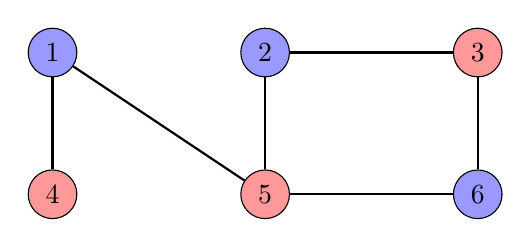
\begin{tikzpicture}[scale=0.9]
\node[draw, circle, fill=blue!40] (1) at (1,3) {$2$};
\node[draw, circle, fill=red!40] (2) at (4,3) {$3$};
\node[draw, circle, fill=red!40] (3) at (1,1) {$5$};
\node[draw, circle, fill=blue!40] (4) at (4,1) {$6$};
\node[draw, circle, fill=red!40] (5) at (-2,1) {$4$};
\node[draw, circle, fill=blue!40] (6) at (-2,3) {$1$};
\path[draw,thick,-] (1) -- (2);
\path[draw,thick,-] (1) -- (3);
\path[draw,thick,-] (3) -- (4);
\path[draw,thick,-] (2) -- (4);
\path[draw,thick,-] (3) -- (6);
\path[draw,thick,-] (5) -- (6);
\end{tikzpicture}
\end{center}

Verkko on kaksijakoinen tarkalleen silloin,
kun siinä ei ole sykliä, johon kuuluu
pariton määrä solmuja.

\subsubsection{Yksinkertaisuus}

Verkko on yksinkertainen (\textit{simple}),
jos mistään solmusta ei ole kaarta itseensä
eikä minkään kahden solmun välillä ole
monta kaarta samaan suuntaan.
Usein oletuksena on, että verkko on yksinkertainen.

Esimerkiksi verkko
\begin{center}
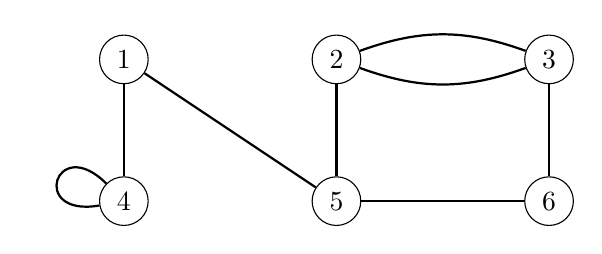
\begin{tikzpicture}[scale=0.9]
\node[draw, circle] (1) at (1,3) {$2$};
\node[draw, circle] (2) at (4,3) {$3$};
\node[draw, circle] (3) at (1,1) {$5$};
\node[draw, circle] (4) at (4,1) {$6$};
\node[draw, circle] (5) at (-2,1) {$4$};
\node[draw, circle] (6) at (-2,3) {$1$};

\path[draw,thick,-] (1) edge [bend right=20] (2);
\path[draw,thick,-] (2) edge [bend right=20] (1);
%\path[draw,thick,-] (1) -- (2);
\path[draw,thick,-] (1) -- (3);
\path[draw,thick,-] (3) -- (4);
\path[draw,thick,-] (2) -- (4);
\path[draw,thick,-] (3) -- (6);
\path[draw,thick,-] (5) -- (6);

\tikzset{every loop/.style={in=135,out=190}}
\path[draw,thick,-] (5) edge [loop left] (5);
\end{tikzpicture}
\end{center}
ei ole yksinkertainen, koska solmusta 4 on kaari itseensä
ja solmujen 2 ja 3 välillä on kaksi kaarta.

\section{Verkko muistissa}

On monia tapoja pitää verkkoa muistissa algoritmissa.
Sopiva tietorakenne riippuu siitä,
kuinka suuri verkko on ja
millä tavoin algoritmi käsittelee sitä.
Seuraavaksi käymme läpi kolme tavallista vaihtoehtoa
käyttäen esimerkkinä seuraavaa verkkoa:
\begin{center}
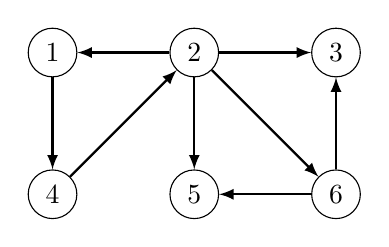
\begin{tikzpicture}[scale=0.9]
\node[draw, circle] (1) at (1,3) {$1$};
\node[draw, circle] (2) at (1,1) {$4$};
\node[draw, circle] (3) at (3,3) {$2$};
\node[draw, circle] (4) at (5,3) {$3$};
\node[draw, circle] (5) at (3,1) {$5$};
\node[draw, circle] (6) at (5,1) {$6$};

\path[draw,thick,->,>=latex] (1) -- (2);
\path[draw,thick,->,>=latex] (2) -- (3);
\path[draw,thick,->,>=latex] (3) -- (1);
\path[draw,thick,->,>=latex] (3) -- (4);
\path[draw,thick,->,>=latex] (3) -- (5);
\path[draw,thick,->,>=latex] (3) -- (6);
\path[draw,thick,->,>=latex] (6) -- (4);
\path[draw,thick,->,>=latex] (6) -- (5);
\end{tikzpicture}
\end{center}

\subsubsection*{Vieruslistat}

Yleisin tapa pitää verkkoa muistissa
on käyttää vieruslistaesitystä.
Siinä jokaisella solmulla on vieruslista (\textit{adjacency list}),
joka kertoo, mihin solmuihin siitä pääsee suoraan kaarella.
Useimmat verkkoalgoritmit pystyy toteuttamaan tehokkaasti
käyttäen vieruslistaesitystä.

Vieruslistoja varten voi luoda esimerkiksi taulukon vektoreita
\begin{lstlisting}
vector<int> v[N];
\end{lstlisting}
minkä jälkeen kaaret voi lisätä näin:
\begin{lstlisting}
v[1].push_back(4);
v[2].push_back(1);
v[2].push_back(3);
v[2].push_back(5);
v[2].push_back(6);
v[4].push_back(2);
v[6].push_back(3);
v[6].push_back(5);
\end{lstlisting}

Taulukon koko $N$ on valittu niin suureksi,
että taulukossa on oma vieruslista
jokaiselle verkossa esiintyvälle solmulle.

Vieruslistaesityksen avulla voi käydä tehokkaasti
läpi kaikki tietystä solmusta lähtevät kaaret.
Se onnistuu seuraavasti solmulle $s$:
\begin{lstlisting}
for (int i = 0; i < v[s].size(); i++) {
    // käsittele solmu v[s][i]
}
\end{lstlisting}

Jos verkon kaarilla on painot,
vieruslistat voi rakentaa esimerkiksi niin,
että jokainen listan solmu on pari,
jossa on solmun tunnus ja siihen johtavan kaaren paino.
Tällöin verkon määrittelystä tulee
\begin{lstlisting}
vector<pair<int,int>> v[N];
\end{lstlisting}
ja esimerkiksi kaari solmusta 2 solmuun 5 painolla 4 lisätään näin:
\begin{lstlisting}
v[2].push_back({5,4});
\end{lstlisting}

\subsubsection*{Vierusmatriisi}

Vierusmatriisi (\textit{adjacency matrix})
kertoo jokaisesta kaaresta,
onko se mukana verkossa.
Matriisista on tehokasta tarkistaa,
onko kahden solmun välillä kaari,
mutta toisaalta matriisi vie paljon tilaa,
jos verkko on suuri.

Vierusmatriisi on yleensä järkevää tallentaa
taulukkona

\begin{lstlisting}
int v[N][N];
\end{lstlisting}

jossa \texttt{v}[$a$][$b$] on 1,
jos solmusta $a$ on kaari solmuun $b$, ja muuten 0.
Seuraava koodi lisää esimerkin kaaret verkkoon:
\begin{lstlisting}
v[1][4] = 1;
v[2][1] = 1;
v[2][3] = 1;
v[2][5] = 1;
v[2][6] = 1;
v[4][2] = 1;
v[6][3] = 1;
v[6][5] = 1;
\end{lstlisting}

Jos verkko on painotettu, luvun 1 sijasta
vierusmatriisin voi tallentaa luontevasti
kyseisen kaaren painon.

\subsubsection*{Kaarilista}

Kaarilista (\textit{edge list}) sisältää kaikki verkon kaaret.
Kaarilista on hyvä tapa tallentaa verkko,
jos algoritmissa täytyy käydä läpi
kaikki verkon kaaret eikä ole tarvetta
etsiä kaarta alkusolmun perusteella.

Kaarilistan voi tallentaa esimerkiksi vektoriin
\begin{lstlisting}
vector<pair<int,int>> v;
\end{lstlisting}
jossa jokaisessa solmussa on parina kaaren
alku- ja loppusolmu.
Kaaret lisätään listalle näin:

\begin{lstlisting}
v.push_back(make_pair(1,4));
v.push_back(make_pair(2,1));
v.push_back(make_pair(2,3));
v.push_back(make_pair(2,5));
v.push_back(make_pair(2,6));
v.push_back(make_pair(4,2));
v.push_back(make_pair(6,3));
v.push_back(make_pair(6,5));
\end{lstlisting}

Toinen tapa toteuttaa kaarilista
on tallentaa tiedot kaarten alku-
ja loppusolmuista taulukkoihin
seuraavaan tapaan:

\begin{lstlisting}
a[1] = 1; b[1] = 4;
a[2] = 2; b[2] = 1;
a[3] = 2; b[3] = 3;
a[4] = 2; b[4] = 5;
a[5] = 2; b[5] = 6;
a[6] = 4; b[6] = 2;
a[7] = 6; b[7] = 3;
a[8] = 6; b[8] = 5;
\end{lstlisting}
% 
% \subsubsection*{Epäsuora esitys}
% 
% Joskus verkkoa on kätevää käsitellä epäsuoran
% esityksen (\textit{implicit representation}) kautta.
% Tämä tarkoittaa, että muistissa ei ole
% suoraan verkon solmuja ja kaaria
% vaan verkko on kuvattu jollakin
% toisella tavalla.
% 
% Tyypillinen esimerkki epäsuorasta
% verkosta on labyrintti:
% \\
% \begin{center}
% \begin{tikzpicture}[scale=0.7]
% \fill[color=gray] (0,0) rectangle (8,1);
% \fill[color=gray] (0,5) rectangle (8,6);
% \fill[color=gray] (0,0) rectangle (1,6);
% \fill[color=gray] (7,0) rectangle (8,6);
% 
% \fill[color=gray] (2,0) rectangle (3,4);
% \fill[color=gray] (4,2) rectangle (6,4);
% 
% \draw (0,0) grid (8,6);
% 
% \node at (1.5,1.5) {$a$};
% \node at (6.5,3.5) {$b$};
% \end{tikzpicture}
% \end{center}
% ~\\
% Labyrintti vastaa verkkoa,
% jossa jokainen lattiaruutu on solmu
% ja vierekkäisten lattiaruutujen
% välissä on kaari.
% Verkko näyttää tältä:
% \\
% \begin{center}
% \begin{tikzpicture}[scale=0.7]
% \node[draw,circle,minimum size=20pt] (a) at (1,1) {$a$};
% \node[draw,circle,minimum size=20pt] (b) at (1,2.5) {};
% \node[draw,circle,minimum size=20pt] (c) at (1,4) {};
% \node[draw,circle,minimum size=20pt] (d) at (1,5.5) {};
% \node[draw,circle,minimum size=20pt] (e) at (2.5,5.5) {};
% \node[draw,circle,minimum size=20pt] (f) at (4,5.5) {};
% \node[draw,circle,minimum size=20pt] (g) at (5.5,5.5) {};
% \node[draw,circle,minimum size=20pt] (h) at (7,5.5) {};
% \node[draw,circle,minimum size=20pt] (i) at (8.5,5.5) {};
% \node[draw,circle,minimum size=20pt] (j) at (8.5,4) {$b$};
% \node[draw,circle,minimum size=20pt] (k) at (8.5,2.5) {};
% \node[draw,circle,minimum size=20pt] (l) at (8.5,1) {};
% \node[draw,circle,minimum size=20pt] (m) at (7,1) {};
% \node[draw,circle,minimum size=20pt] (n) at (5.5,1) {};
% \node[draw,circle,minimum size=20pt] (o) at (4,1) {};
% \node[draw,circle,minimum size=20pt] (p) at (4,2.5) {};
% \node[draw,circle,minimum size=20pt] (q) at (4,4) {};
% 
% \path[draw,thick,-] (a) -- (b);
% \path[draw,thick,-] (b) -- (c);
% \path[draw,thick,-] (c) -- (d);
% \path[draw,thick,-] (d) -- (e);
% \path[draw,thick,-] (e) -- (f);
% \path[draw,thick,-] (f) -- (g);
% \path[draw,thick,-] (g) -- (h);
% \path[draw,thick,-] (h) -- (i);
% \path[draw,thick,-] (i) -- (j);
% \path[draw,thick,-] (j) -- (k);
% \path[draw,thick,-] (k) -- (l);
% \path[draw,thick,-] (l) -- (m);
% \path[draw,thick,-] (m) -- (n);
% \path[draw,thick,-] (n) -- (o);
% \path[draw,thick,-] (o) -- (p);
% \path[draw,thick,-] (p) -- (q);
% \path[draw,thick,-] (q) -- (f);
% \end{tikzpicture}
% \end{center}
% ~\\
% Kätevä tapa tallentaa labyrintti on luoda taulukko
% merkkijonoista. Jokainen merkkijono vastaa yhtä
% labyrintin riviä:
% \begin{lstlisting}
% s[0] = "########";
% s[1] = "#......#";
% s[2] = "#.#.##b#";
% s[3] = "#.#.##.#";
% s[4] = "#a#....#";
% s[5] = "########";
% \end{lstlisting}
